%% content.tex
%%

%% ==============
\chapter{Grundlagen}
\label{ch:Grundlagen}
%% ==============
\section{Rasterelektronenmikroskop}
\label{ch:Grundlagen:sec:REM}
In Abbildung \ref{fig:aufbau_rem} ist schematisch der Aufbau eines Rasterelektronenmikroskops~(REM) dargestellt. Aus in einer Elektronenquelle werden durch eine Spannung $U_{B}$ von einigen kV Elektronen (Prim"ar Elektronen - PE) aus einer Kathode gel"ost und beschleunigt. Durch ein System aus Magnetlinsen, Ablenkspulen und Blenden wird ein Elektronenstrahl geformt, mit dem die eine Probe abgetastet werden kann. Treffen PE auf die Probe werden diese durch elastische oder inelastische Streuung abgebremst. \todo{mehr.. hab keine lust mehr}


\begin{figure}%
\centering
\begin{adjustwidth}{-1.5cm}{0cm}
	\subfloat[Ionisationsbirne \cite{Reimer}.]{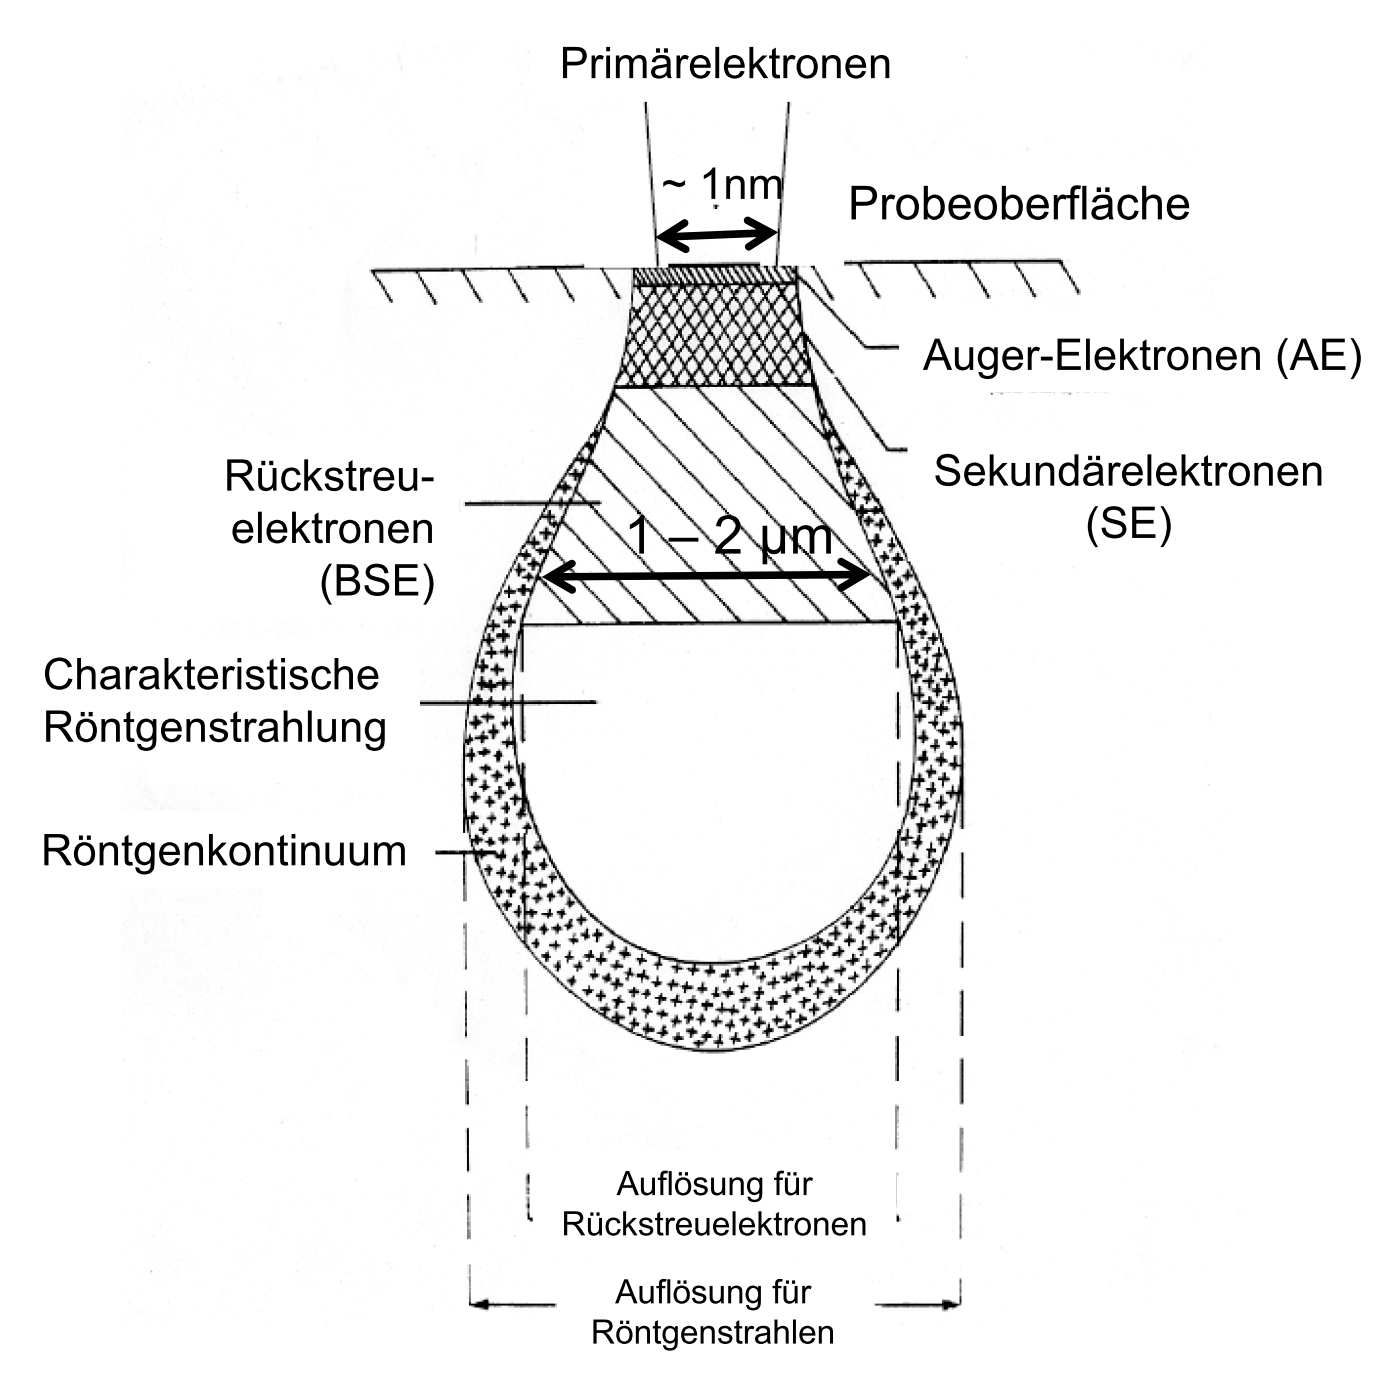
\includegraphics[width=.6\columnwidth]{Grafiken/ionisationsbirne.jpg}\label{fig:ionisationsbirne}}
	\subfloat[Schematischer Aufbau eines REMs \cite{Colliex}.]{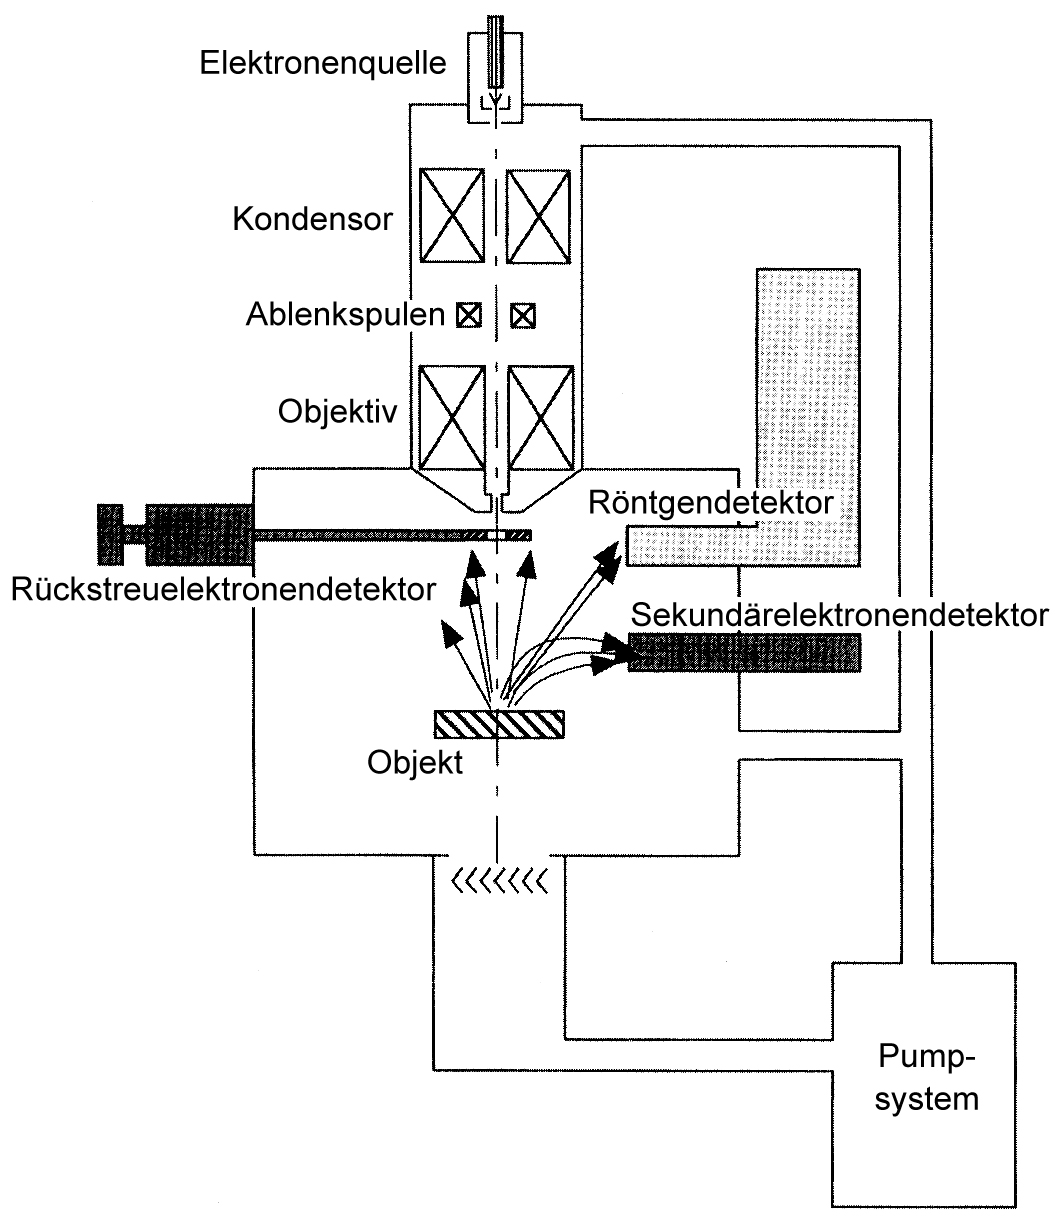
\includegraphics[width=.6\columnwidth]{Grafiken/rem-schema-1.jpg} \label{fig:aufbau_rem}}%
	\end{adjustwidth}
\caption{bla.}%
\label{fig:rem_subfig}%
\end{figure}




%
%\begin{figure}
%\centering
%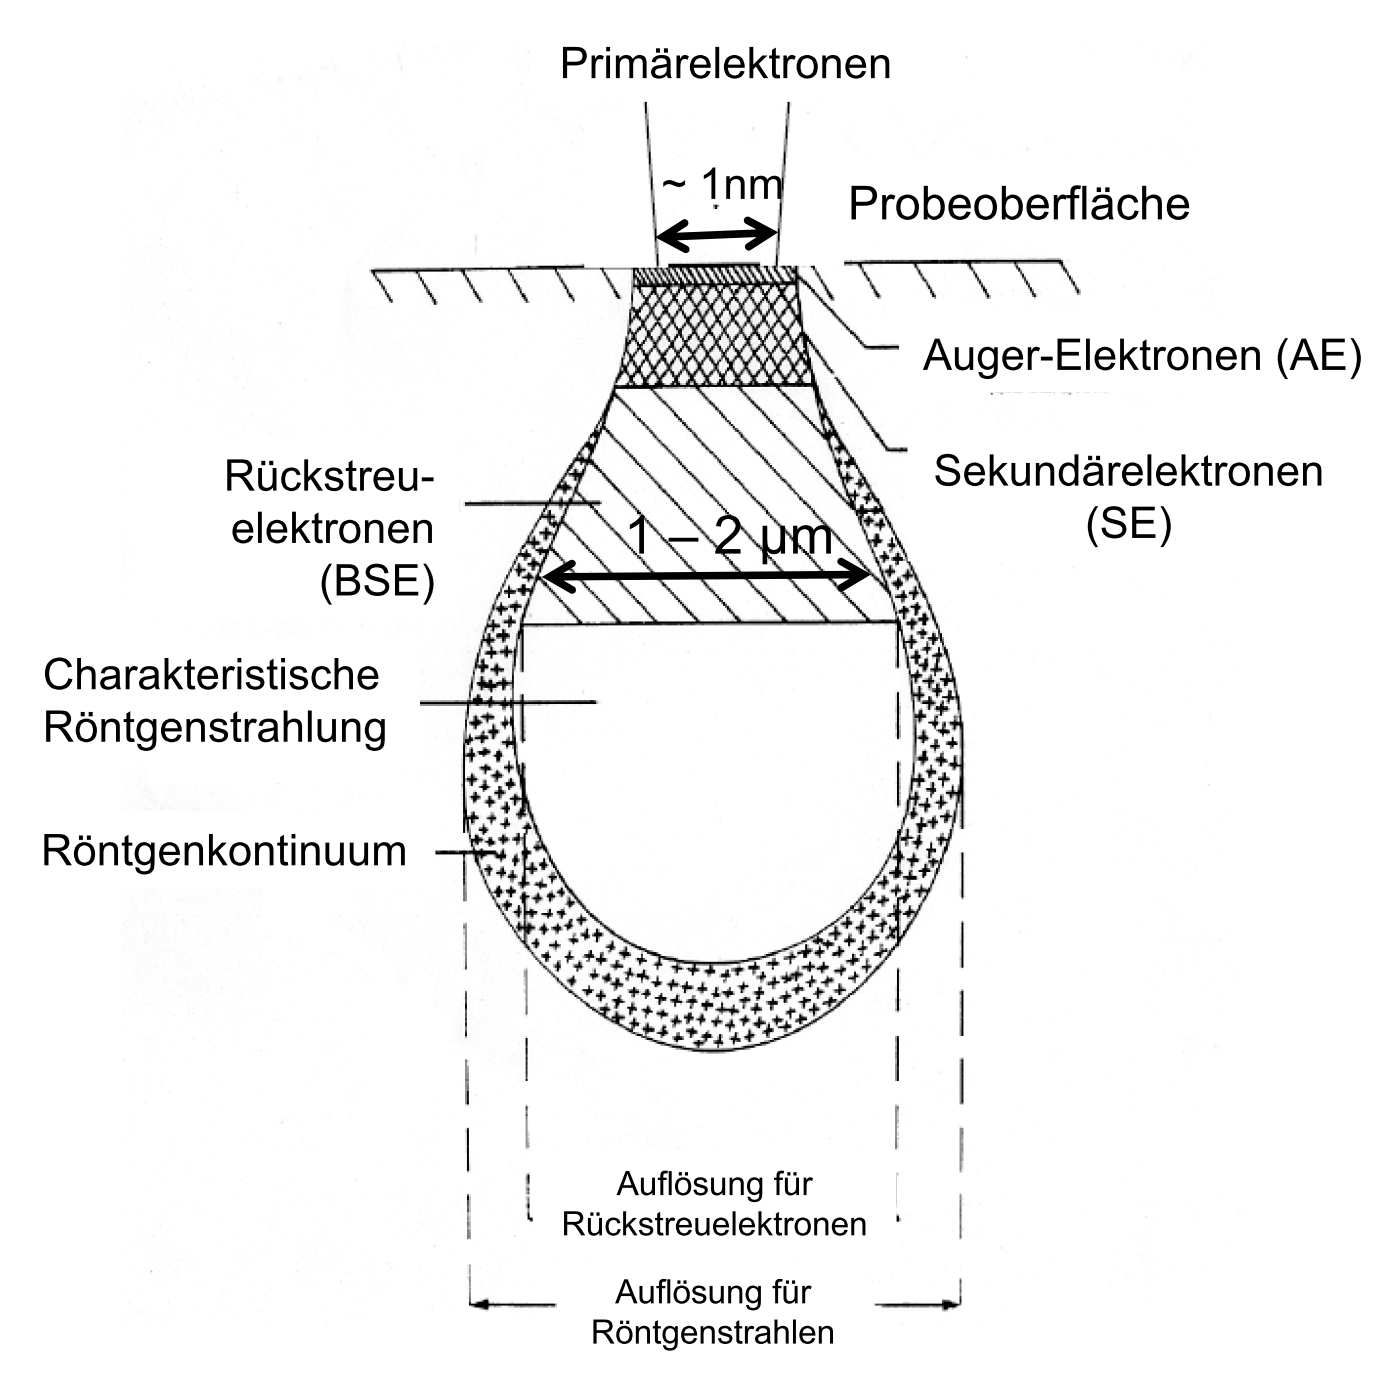
\includegraphics[width=.5\columnwidth]{Grafiken/ionisationsbirne.jpg}%
%\caption{Ionisationsbirne \cite{Reimer}.}
%\label{fig:ionisationsbirne}
%\end{figure} 
%
%\begin{figure}
%\centering
%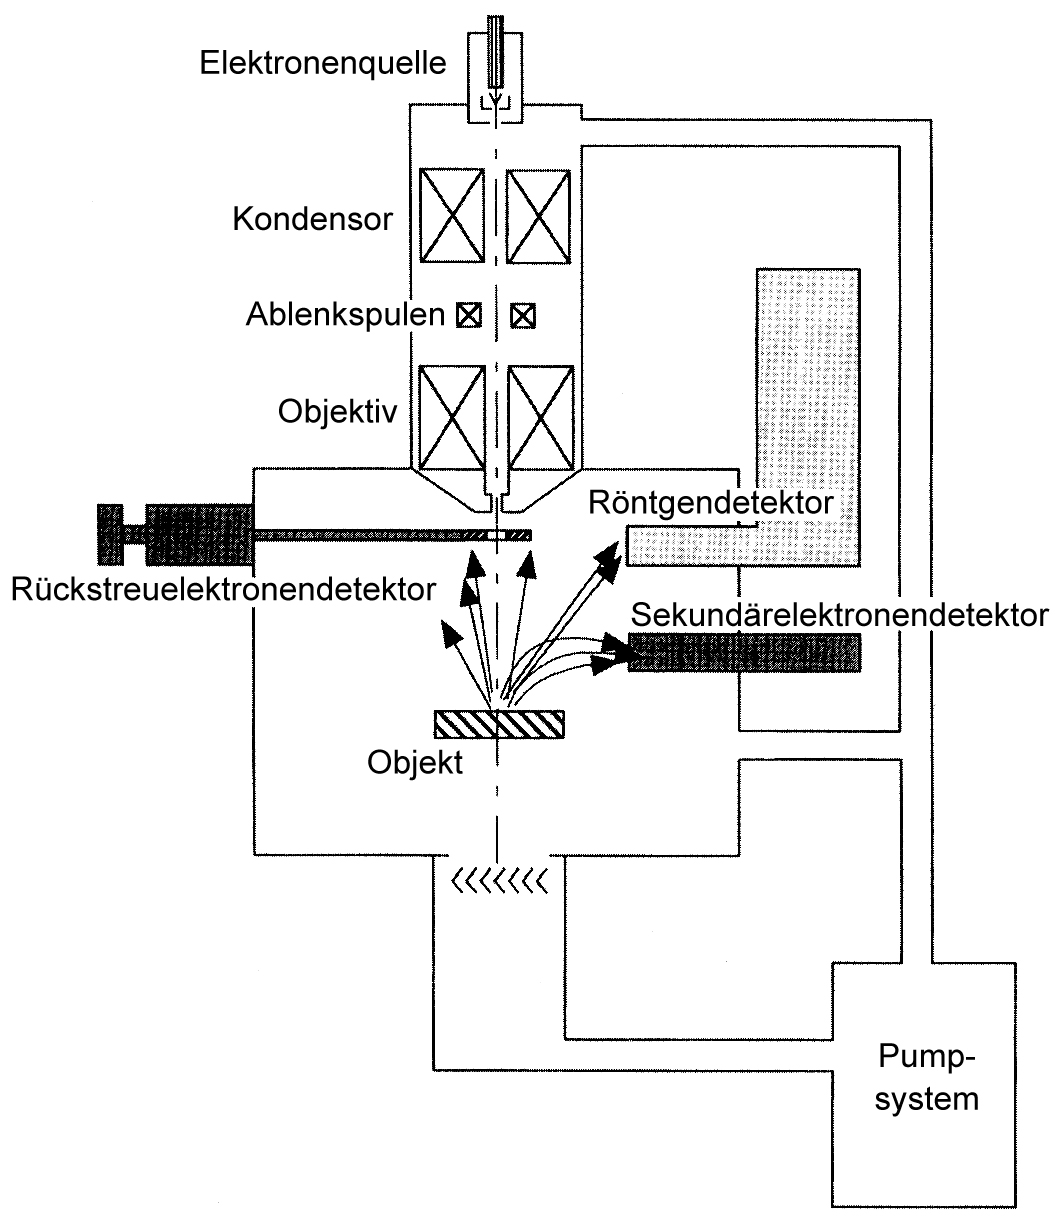
\includegraphics[width=.5\columnwidth]{Grafiken/rem-schema-1.jpg}%
% 
%\caption{Schematischer Aufbau eines REMs \cite{Colliex}.}
%\label{fig:aufbau_rem}
%\end{figure} 

\subsection{Aufbau}
\label{ch:Grundlagen:sec:REM:sub:Aufbau}

\subsection{Aufl�sungsverm�gen}
\label{ch:Grundlagen:sec:REM:sub:Aufl�sung}

\subsection{Tiefensch�rfe}
\label{ch:Grundlagen:sec:REM:sub:Tiefenschaerfe}

\section{Direct Laser Writing}
\label{ch:DLW}

\section{Aufbau und Funktionsweise}
\label{ch:DLW:sec:Aufbau}

\section{Noch eine}
\label{ch:DLW:sec:bla}

%% ===========================
\chapter{Versuchsdurchf�hrung}
\label{ch:Durchfuerhung}

\section{Probenherstellung}
\label{ch:Durchfuerhung:sec:Herstellung}

Zur Herstellung der Proben wurde auf ein gereinigtes Glassubstrat mit einem \textit{Spin Coater} ein Fotolackfilm (SU-8) aufebracht. Um das L�sungsmittel aus dem Lack zu treiben, wurde die Probe bei 95~�C auf einer \textit{Hot Plate} gebacken (\textit{Soft Bake}) \cite{Versuchsanleitung}. Diese Probenvorbereitung erfolgte durch den Versuchsbetreuer.

\todo{Schreiben der Probe im DLW}

Nach der Belichtun des Fotolacks erfolgte ein $Post~Exposure~Bake$ (PEB) f�r 7 Minuten bei 95~�C auf einer $Hot~Plate$. Bei diesem Backvorgang werden zuvor belichtete Bereiche des Lacks quervernetzt und damit unempfindlich gegen�ber dem Entwickler. Anschlie�end erfolgte die Entwicklung mit dem Entwickler \mbox{mr-Dev 600}. 
Die Probe wurde f�r 7 Minuten im Entwickler geschwenkt, zum stoppen der Entwicklung mit Isopropanol abgesp�hlt und mit Stickstoff getrocknet. Nach einer optischen Kontrolle der Probe wurde die Probe f�r eine weitere Minute in \mbox{mr-Dev 600} nachentwickelt. Bei der Entwicklung werden die zuvor nicht belichteten Lackbereiche entfernt.

Um die Lackstrukturen weiter zu festigen wurde die Probe f�r 10 Minuten bei 150~�C auf einer $Hot~Plate$ gebacken ($Hard Bake$). Bei diesem $Hard~Bake$ werden au�erdem Isopropanolreste aus den Strukturen ausgetrieben. Dies ist notwendig, damit beim sp�ter durchgef�hrten Aufsputtern von Gold zu keiner Zerst�rung der Strukturen durch das Plasma kommt.

Die Abscheidung von Gold erfolgte in einer Hochfrequenz (engl. $radio~frequency$ - RF)-Sputteranlage durchgef�hrt. Die Goldschicht dient dazu Aufladungseffekte auf den nicht leitf�higen Lackstrukuturen w�hrend dem Betrachten unter dem REM zu verhindern.
 


\section{evtl. noch was}
\label{ch:Durchfuerhung:sec:keine}

\chapter{Auswertung der Messergebnisse}
\label{ch:Auswertung}

\section{Bestimmung der Voxelgr��e}
\label{ch:Auswertung:sec:voxel}

Um die Voxelausdehnung in z-Richtung zu bestimmen, wurden einzelne Voxel nebeneinander geschrieben. Hierbei wurde die Position in z-Richtung mit jedem Voxel um 100~nm erh�ht. Abbildung \ref{fig:steigung} zeigt dies Schematisch. Der Laser ist zuerst in das Glassubstrat fokusiert. Der Fokus verschiebt sich mit jedem Voxel nach oben. Sobald sich der Fokus im Fotolack befindet, wird dieser belichtet. Nach dem Entwickeln verbleiben nur die Voxel stehen, die direkten Kontakt zum Glassubstrat haben. In Abbildung \ref{fig:steigung} w�rde somit der erste Laserfokuspunkt kein Voxel bilden, das Voxel des letzten Fokuspunktes w�rde beim Entwickeln wegschwimmen. Aus der Anzahl der verbleibenden Voxel l�sst sich damit Voxelausdehnung in z-Richtung absch�tzen.

Abbildung \ref{fig:voxelausdehnung} zeigt eine REM-Aufnahme der geschriebenen Voxelstrukturen. Es wurde Laserleistung von 1,75~mW verwendet. Die Belichtungszeit pro Voxel steigt von betr�gt (Zeilenweise, von unten nach oben) 10~ms, 20~ms und 30~ms. In der untersten Reihe sind 8 Voxel zu erkennen. Daraus l�sst sich eine Voxelausdehnung in z-Richtung von $\sim800$~nm absch�tzen. In Tabelle \ref{tab:Ausdehnung} sind die Voxelgr��en in Abh�ngigkeit der Energie zu finden.

Um die Voxelausdehnung in x- bzw. y-Richtung zu bestimmen, wurde das jeweils letzte Voxel einer Reihe vermessen. Bei diesen Voxeln ist bei einer Aufsicht die volle Voxelbreite zu messen. Abbildung \ref{fig:voxel_x} zeigt die Aufsicht auf ein Voxel (Laserleistung: 1,75~W, Belichtungszeit: 30~ms). Zu erkennen ist eine elliptische Form. Zu erwarten w�re eine kreisf�rmige Form \cite{Multiphoton}. Dies ist vermutlich auf eine astigmatische Aberration des Linsensystems beim Schreiben der Strukturen zur�ckzuf�hren. 
Zur Bestimmung der Voxelbreite wurde die k�rzere Achse der Ellipse gew�hlt. F�r das in der Abbildung gezeigte Voxel ergibt sich damit eine laterale breite von $\sim1,14$~$\upmu$m.

\begin{figure}%
\centering
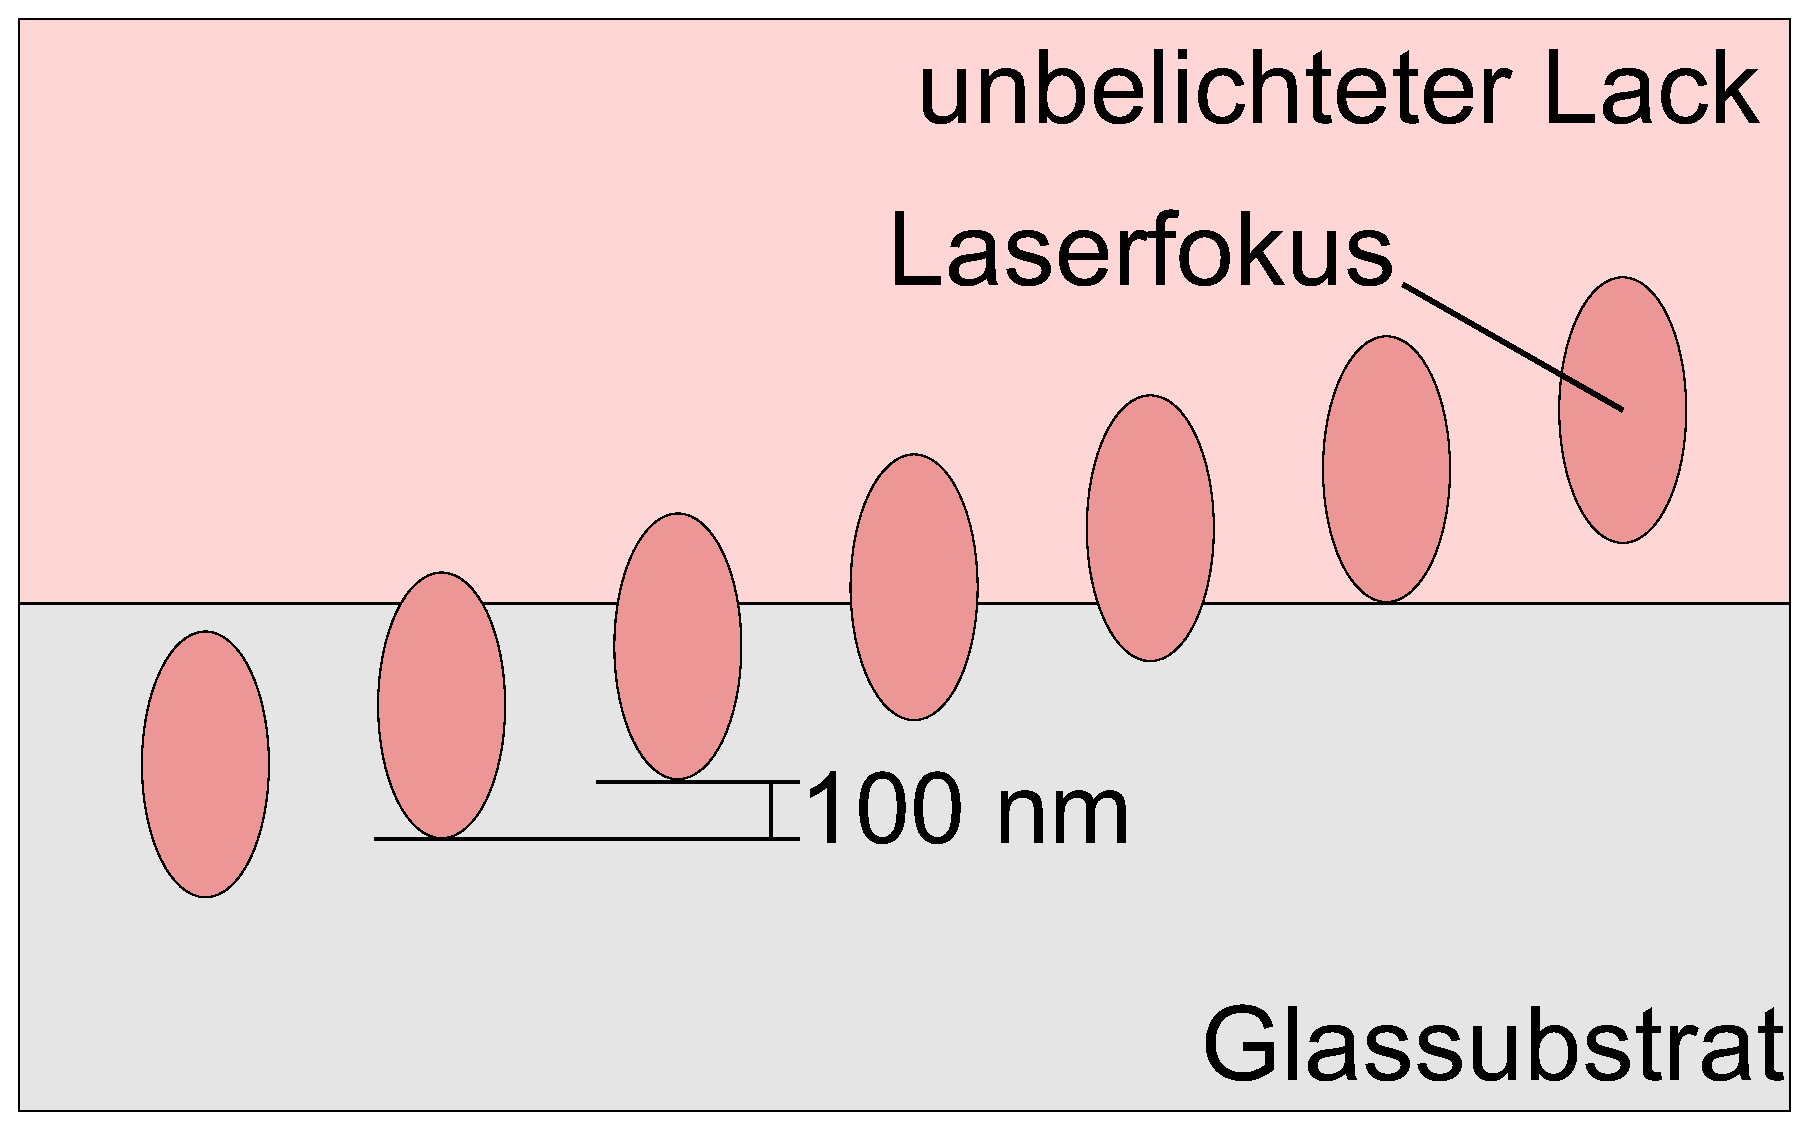
\includegraphics[width=.5\columnwidth]{Grafiken/Steigung.pdf}%
\caption{Schematische Darstellung: Bestimmung der Voxelausdehnung in z-Richtung.}%
\label{fig:steigung}
\end{figure}

%\begin{figure}%
%\centering
%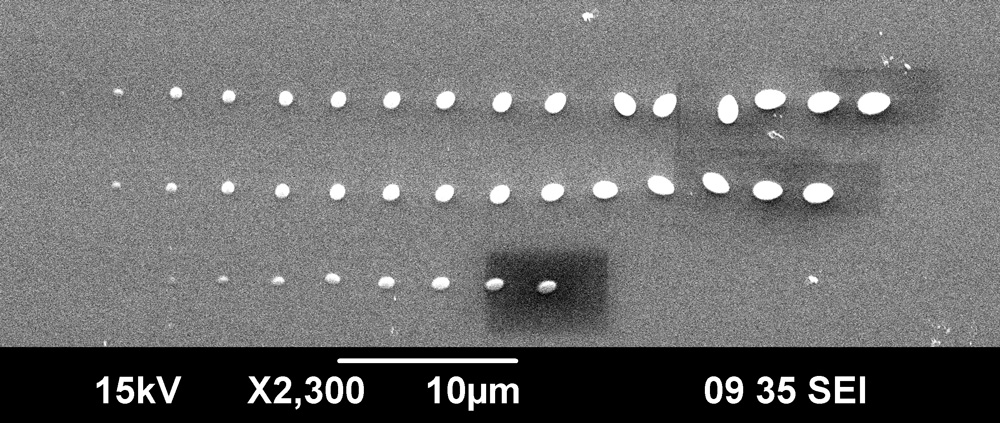
\includegraphics[width=.8\columnwidth]{Grafiken/voxel_bsp.jpg}%
%\caption{REM Aufnahme der Voxelstrukturen.}%
%\label{fig:voxelausdehnung}%
%\end{figure}
%



\begin{figure}%
\centering
\begin{adjustwidth}{-.5cm}{0cm}
	\subfloat[Voxelanordnung]{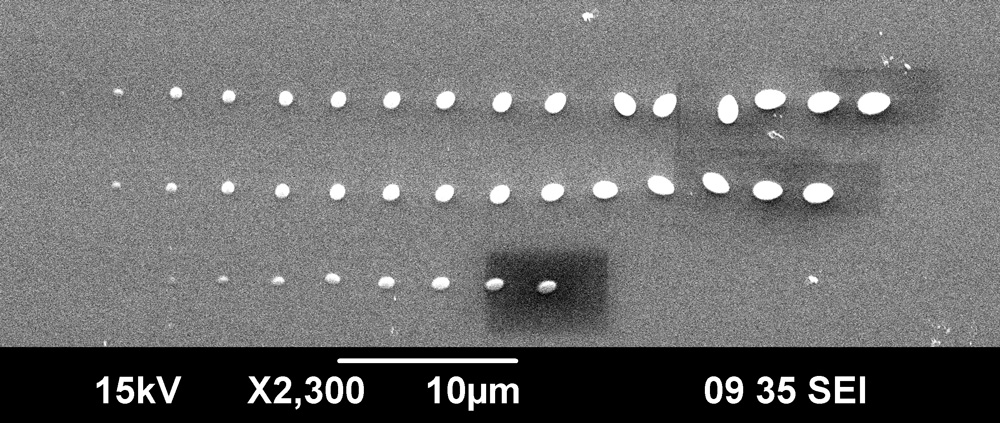
\includegraphics[totalheight=4 cm]{Grafiken/voxel_bsp.jpg}\label{fig:voxelausdehnung}\qquad}
	\subfloat[Voxelgr��e]{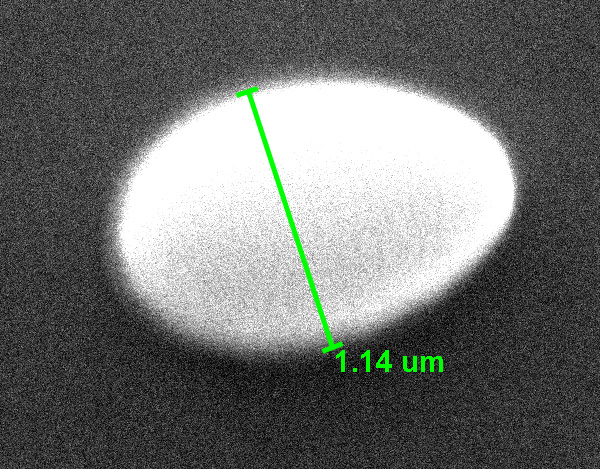
\includegraphics[totalheight=4 cm]{Grafiken/voxel_x.jpg} \label{fig:voxel_x}}%
\end{adjustwidth}
\caption{REM Aufnahmen der Voxelstrukturen}%
\label{fig:voxel_subfig}%
\end{figure}

%\begin{figure}%
%\centering
%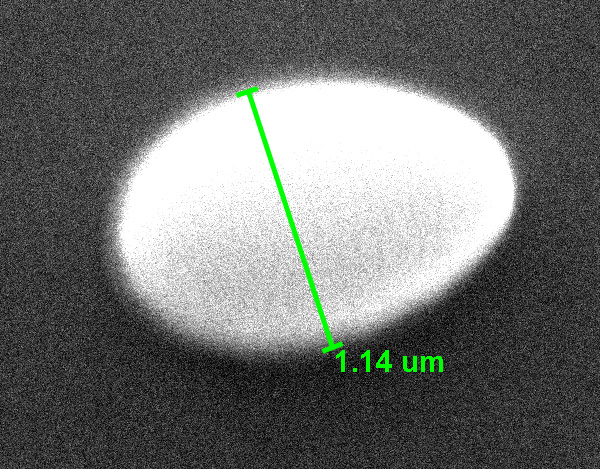
\includegraphics[width=\columnwidth]{Grafiken/voxel_x.jpg}%
%\caption{}%
%\label{}%
%\end{figure}

\section{Bestimmung der Polymerisationsschwelle}
\label{ch:Auswertung:sec:Polymerisation}

\section{Probleme bei Gitterstrukturen}
\label{ch:Auswertung:sec:ProblemeGitter}

\section{Demonstration dreidimensionaler Strukturen}
\label{ch:Auswertung:sec:LTI}



\chapter{Zusammenfassung}
